\documentclass[t]{beamer}

\usepackage[slovene]{babel}
\usepackage[T1]{fontenc}
\usepackage[utf8]{inputenc}
\usepackage{amssymb}
\usepackage{amsmath}


\usepackage{lmodern}                           
\renewcommand\textbullet{\ensuremath{\bullet}}
\title{Krožnica v racionalni Bezierjevi obliki}
\author{Anja Kišek, Samo Kralj}

\usetheme{CambridgeUS}

\begin{document}
%%%%%%%%%%%%%%%%%%%%%%%%%%%%%%%%%%%%%%
\begin{frame}
\titlepage
\end{frame}

%%%%%%%%%%%%%%%%%%%%%%%%%%%%%%%%%%%%%

\begin{frame}
Vsebina:
\begin{itemize}
\item Definicija racionalnih Bezierjevih krivulj

\item Konstrukcija sklenjene krožnice s krivuljami stopnje 2,3,4

\item Krožni loki v racionalni Bezierjevi obliki

\item Kubični polkrogi

\end{itemize}

\end{frame}
%%%%%%%%%%%%%%%%%%%%%%%%%%%%%%%%%%%%
\begin{frame}
Racionalna Bezierjeva krivulja $C(t)$ stopnje $n$ v $\mathbb{R}^d$ je projekcija polinomske Bezierjeve krivulje $\tilde{C}(t)$stopnje $n$ v $\mathbb{R}^{d+1}$ na hiperravnino $w=1$, kjer je točka v $\mathbb{R}^{d+1}$ označena z $
\begin{bmatrix} x \\ w \end{bmatrix}.$


Racionalna B. krivulja stopnje $n$ je tako podana s predpisom
$$r(t) = \frac{\sum_{i=0}^n w_ib_iB_i^n(t)}{\sum_{i=0}^n w_iB_i^n(t)} $$

\end{frame}
%%%%%%%%%%%%%%%%%%%%%%%%%%%%%
\begin{frame}
Racionalna krivulja $C(t) = (X(t), Y(t))$ lahko eksaktno opiše krožnico kot projekcijo krivulje
$\tilde{C}(t) = (\tilde{X}(t), \tilde{Y}(t), W(t)),$ ki leži na stožcu, na ravnino $w = 1$.

\begin{align*}
X(t)^2 + Y(t)^2 &= 1 \\
\Big{(}\frac{\tilde{X}(t)}{W(t)}\Big{)}^2 + \Big{(}\frac{\tilde{Y}(t)}{W(t)}\Big{)}^2 &= 1\\
\tilde{X}(t)^2 + \tilde{Y}(t)^2 - W(t)^2 &= 0
\end{align*}
\begin{figure}
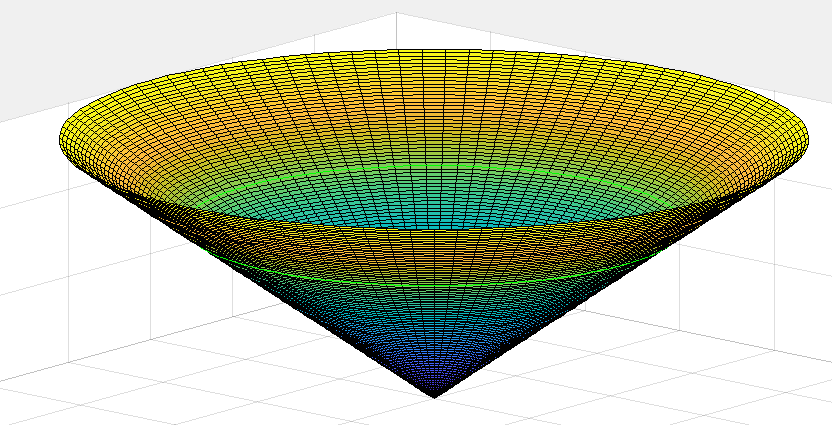
\includegraphics[scale=0.2]{stozec.png}
\end{figure}

\end{frame}

%%%%%%%%%%%%%%%%%%%%%%%%%%%%%

\begin{frame}
\textbf{Bezierjeva krivulja kot sklenjena krožnica}

Ali lahko krožnico zapišemo kot racionalno Bezierjevo krivuljo določene stopnje?
\begin{itemize}
\item Kvadratična krivulja: Ne

Zlepek krožnih lokov s kontrolnimi točkami:
\begin{align*}
\tilde{P}_0 &= (cos(\phi), -sin(\phi), 1)\\
\tilde{P}_1 &= (1, 0, cos(\phi))\\
\tilde{P}_2 &= (cos(\phi), sin(\phi), 1)
\end{align*}

\item Kubična krivulja: Ne
\end{itemize}
\end{frame}
%%%%%%%%%%%%%%%%%%%%%%%%%%%%%%%%%%%%%%
\begin{frame}
\begin{itemize}
\item Krivulja 4. stopnje: reševanje sistema 9 enačb
\begin{align*}
\tilde{y}_3 + \tilde{y}_1 &= 0\\
\tilde{x}_3 + \tilde{x}_1 &= 0\\
3\tilde{x}_2 + 4\tilde{y}_1^2 - 3w_3 &= 0 \\
\tilde{x}_1\tilde{x}_2 + \tilde{y}_1\tilde{y}_2  - \tilde{x}_1w_2 &= 0 \\
9\tilde{x}_2^2 - 8\tilde{y}_1^2 + \tilde{y}_2^2 - 9w_2^2&= 0 \\
\end{align*}
Za $\alpha = (\frac{3w_2}{2} - \tilde{x}_1^2 + \frac{1}{2})^{\frac{1}{2}}$ dobimo dva kontrolna poligona
\begin{align*}
\tilde{P}_0 &= (1,0, 1)\\
\tilde{P}_1 &= (\tilde{x}_1, \pm \alpha,\tilde{x}_1)\\
\tilde{P}_2 &= (-\frac{3w_2 - 4\tilde{w}_1^2+2}{3}, \pm \frac{3}{4}\tilde{x}_1\alpha, w_2)\\
\tilde{P}_3 &= (-\tilde{x}_1, \mp \alpha,-\tilde{x}_1)\\
\tilde{P}_4 &= (1,0,1) \\
\end{align*}
\end{itemize}

\end{frame}
%%%%%%%%%%%%%%%%%%%%%%%%%%%%%%%%%
\begin{frame}
\begin{itemize}
\item Krivulja 4. stopnje: uteži so lahko negativne ali ničelne
\item Krivulja 5. stopnje: s pomočjo višanja stopnje

Primer:
\begin{columns}
	\column{0.5\linewidth}
	\begin{align*}
	\tilde{P}_0 &= (1,0, 1)\\
	\tilde{P}_1 &= (0, 1, 0)\\
	\tilde{P}_2 &= (-1, 0, 1/3)\\
	\tilde{P}_3 &= (0, -1, 0)\\
	\tilde{P}_4 &= (1, 0, 1) \\
	\end{align*}
	\column{0.5\linewidth}
    \begin{align*}
	\tilde{P}_0 &= (1,0, 1)\\
	\tilde{P}_1 &= (1/5, 4/5, 1/5)\\
	\tilde{P}_2 &= (-3/5, 2/5, 1/5)\\
	\tilde{P}_3 &= (-3/5, -2/5, 1/5)\\
	\tilde{P}_4 &= (1/5, -4/5, 1/5)\\
	\tilde{P}_5 &= (1, 0, 1) \\
	\end{align*}
\end{columns}

\end{itemize}
\end{frame}

\begin{frame}{Racionalni kubični krožni loki}
Zanima nas, kakšne krožne loke lahko opišemo s kubično racionalno bezierjevo krivuljo pri pogoju, da bodo vse uteži pozitivne.
Kako pridemo do enačb kontrolnih točk?
$$
X(t)^2 + Y(t)^2 - W(t)^2 = 0
$$
\begin{align*}
X(t) &= x_{0} B_{0}^3 (t) + x_{1} B_{1}^3 (t) + x_{2} B_{2}^3 + x_{3} B_{3}^3 = \\
&= x_{0} \binom{3}{0} (1-t)^3 + x_{1} \binom{3}{1} t(1-t)^2 + x_{2} \binom{3}{2} t^2(1-t) + x_{3} \binom{3}{3} t^3
\end{align*}
\end{frame}

\begin{frame}
\begin{align*}
x_{0}(1-t)^3 \cdot 3x_{2}t^2(1-t) &= \\
3x_{0} x_{2} \cdot t^2 (1-t)^4 & = \\
3x_{0}x_{2} \frac{\binom{6}{2}}{\binom{6}{2}} t^2 (1-t)^4 &= \\
3x_{0}x_{2} \frac{1}{15} \binom{6}{2} t^2 (1-t)^4 &= \\
\frac{1}{5} x_{0}x_{2} B_{2}^6(t)
\end{align*}
Poberemo skupaj koeficiente pri vsakem $B_{i}^6$, $i=0,1,2,3,4,5,6$. Ker Bernsteinovi polinomi tvorijo bazo, tako dobimo 7 enačb.
\end{frame}

\begin{frame}{Racionalni kubični krožni loki}
Lahko privzamemo, da sta 
\begin{align*}
\tilde{P_{0}} &= (\cos \theta, - \sin \theta, 1) \\
\tilde{P_{3}} &= (\cos \theta, \sin \theta, 1)
\end{align*}
kjer je $\theta$ polovica loka, ki ga želimo opisat. 
Potrebujemo še 
\begin{align*}
\tilde{P_{1}} = (\tilde{x_{1}}, \tilde{y_{1}}, w_{1}) \\
\tilde{P_{2}} = (\tilde{x_{1}}, \tilde{y_{1}}, w_{1})
\end{align*}

\end{frame}

\begin{frame}{Racionalni kubični krožni loki}
Dobimo sistem 5 enačb za 6 neznank:
$$
w_{1} = \cos \theta \tilde{x_{1}} - \sin \theta  \tilde{y_{1}} 
$$
$$
w_{2} = \cos \theta  \tilde{x_{2}} + \sin \theta  \tilde{y_{2}} 
$$
$$
3(\sin \theta )^{2} \tilde{x_{1}}^2 + 3(\cos \theta )^{2} \tilde{y_{1}}^2 - 4 \sin \theta \tilde{y_{2}} + 6\sin \theta \cos \theta \tilde{x_{1}}\tilde{y_{1}} = 0 
$$
$$
3(\sin \theta )^{2} \tilde{x_{2}}^2 + 3(\cos \theta )^{2} \tilde{y_{2}}^2 + 4 \sin \theta 
\tilde{y_{1}} - 6\sin \theta \cos \theta \tilde{x_{2}}\tilde{y_{2}} = 0 
$$
\begin{align*}
9\sin^{2}\theta \tilde{x_{1}}\tilde{x_{2}} + 9 \cos \theta \sin \theta \tilde{y_{1}}\tilde{x_{2}} -\\ -9\cos \theta \sin \theta \tilde{x_{1}} \tilde{y_{2}} + 9 (1 + \sin^2 \theta) \tilde{y_{1}} \tilde{y_{2}} - 2\sin^2\theta = 0
\end{align*}

\end{frame}


\begin{frame}{Konstrukcija kubične polkrožnice}
Želimo konstruirati polovico krožnice. Spomnimo se enačb za kontrolne točke kubčnih bezierjevih krožnih lokov:

\begin{align*}
w_{1} = \cos \theta \tilde{x_{1}} - \sin \theta  \tilde{y_{1}} \\
w_{2} = \cos \theta  \tilde{x_{2}} + \sin \theta  \tilde{y_{2}} \\
3(\sin \theta )^{2} \tilde{x_{1}}^2 + 3(\cos \theta )^{2} \tilde{y_{1}}^2 - 4 \sin \theta \tilde{y_{2}} + 6\sin \theta \cos \theta \tilde{x_{1}}\tilde{y_{1}} = 0 \\
3(\sin \theta )^{2} \tilde{x_{2}}^2 + 3(\cos \theta )^{2} \tilde{y_{2}}^2 + 4 \sin \theta \tilde{y_{1}} - 6\sin \theta \cos \theta \tilde{x_{2}}\tilde{y_{2}} = 0 \\
9\sin^{2}\theta \tilde{x_{1}}\tilde{x_{2}} + 9 \cos \theta \sin \theta \tilde{y_{1}}\tilde{x_{2}} -\\ -9\cos \theta \sin \theta \tilde{x_{1}} \tilde{y_{2}} + 9 (1 + \sin^2 \theta) \tilde{y_{1}} \tilde{y_{2}} - 2\sin^2\theta = 0
\end{align*}
\end{frame}

\begin{frame}{Konstrukcija kubične polkrožnice}
Vstavimo $\theta = \frac{\pi}{2}$.
\begin{align*}
w_{1} = - \tilde{y_{1}} \\
w_{2} = \tilde{y_{2}} \\
3\tilde{x_{1}}^2 - 4 \tilde{y_{2}} = 0 \\
3 \tilde{x_{2}}^2 + 4 \tilde{y_{1}} = 0 \\
9 \tilde{x_{1}} \tilde{x_{2}} + 18 \tilde{y_{1}} \tilde{y_{2}} - 2 = 0
\end{align*}
\end{frame}
\begin{frame}{Konstrukcija kubične polkrožnice}
Označimo $\alpha = \frac{3\tilde{x_{1}}}{2}$ in dobimo rešitev:

\begin{columns}
\column{0.5\linewidth}
\begin{align*}
\tilde{P_{0}} &= (0,-1,1) \\
\tilde{P_{1}} &= (\frac{2\alpha}{3},-\frac{1}{3\alpha^2},\frac{1}{3\alpha^2}) \\
\tilde{P_{2}} &= (\frac{2}{3\alpha},\frac{\alpha^2}{3}, \frac{\alpha^2}{3}) \\
\tilde{P_{3}} &= (0, 1,1)
\end{align*}
\column{0.5\linewidth}
\begin{align*}
P_{0} &= (0,1) \\
P_{1} &= (2\alpha^3, -1) \\
P_{2} &= (\frac{2}{\alpha^3}, 1) \\
P_{3} &= (0, 1) \\
w &= (1, \frac{1}{3\alpha^2}, \frac{\alpha^2}{3}, 1)
\end{align*}
\end{columns}

\end{frame}
\begin{frame}{Konstrukcija kubične polkrožnice}
\begin{itemize}
\item Narišemo premici $y=1$ in $y = -1$
\item Potegnemo poljubno tangento na enotsko krožnico
\item Z $x_{1}$ in $x_{2}$ označimo presečišča te tangente z $y=1$ in $y=-1$.
\item Točke $(0,-1), (2x_{1}, -1), (2x_{2}, 1)$ in $(0,1)$ so kontrolne točke racionalne bezierjeve krivulje, ki nariše polovico krožnice, skupaj z utežmi $(1, \frac{1}{3x_{1}^{2/3}}, \frac{1}{3x_{2}^{2/3}}, 1)$.

\end{itemize}
\end{frame}


\end{document}
